\documentclass[tikz, border = 10pt]{standalone}

\renewcommand{\familydefault}{\sfdefault}

\usetikzlibrary{positioning, calc, quotes, arrows.meta, shapes}

\tikzset{
  every edge quotes/.style = {fill = white},
  > = {Stealth[length = 1.5mm]},
  shorten > = 1pt, 
  shorten < = 1pt, 
  manifest/.style = {draw, inner sep = 3pt, align = center, 
    minimum width = 1cm, minimum height = 0.85cm},
  latent/.style = {manifest, ellipse},
  residual/.style n args = {3}{inner sep = #1, minimum size = #2, #3},
  residual/.default = {0}{0}{},
  constant/.style = {draw, inner sep = 1pt, minimum size = 5mm, 
    regular polygon, regular polygon sides = 3},
  regression/.style = {->, shorten < = 0pt, inner sep = 1.5pt},
  covariance/.style n args = {3}{<->, inner sep = 1.5pt, bend #1 = #2, looseness = #3},
  variance/.style n args = {3}{covariance = {#1}{#2}{#3}, inner sep = 0.5pt}
}

\begin{document}
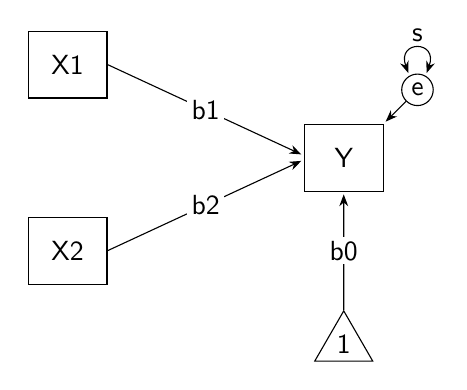
\begin{tikzpicture}

%% Manifest
\node [manifest] (x1) {X1};
\node [manifest] (x2) [below = 1.5cm of x1] {X2};
\node [manifest] (y) [right = 3cm of $ (x1) !0.5! (x2) $] {Y};

%% Regressions
\path [regression] (x1.0) edge ["b1"] (y.177)
                   (x2.0) edge ["b2"] (y.183);

%% Residual
\node [residual = {0}{4mm}{draw, circle}] (e) [above right = 4mm of y] {e};
\path [regression] (e) edge (y.north east);
\path [variance = {right}{110}{6}] (e.60) edge ["s" {above = 2pt}] (e.120);

%% Intercept
\node [constant] (m) [below = 1.5cm of y] {1};
\path [regression] (m) edge ["b0"] (y);

\end{tikzpicture}
\end{document}
